\chapter{Feasibility}
This system needs requirements listed below:
\begin{itemize}
    \item This system needs real time location of user. So this system needs to run on mobile devices.
    \item This system must provide interaction within users. So to provide intraction of multiple mobile devices this system needs a server side application.
    \item In process of development to provide version controlling Git must used as VCS.
\end{itemize}

\section{Technic Feasibility}
As technical feasibility study, the software and hardware needs for the project is defined on the following sections.
\subsection{Software Feasibility}

In this project a web and a mobile application will be developed. The following software
technologies will be used.

\textbf{Mobile Side Development}
\newline
The tools and development environments used for mobile side development of the
project are mentioned below.
\newline
\newline
• Android: Android is a mobile operating system based on the Linux kernel. Its
source code is licensed under open source licenses and it is developing by Google
and Open Handset Alliance. The top layer of Android’s architecture is called
The Application Framework layer and it provides many higher-level services to
applications in the form of Java classes. Android was chosen over iOS because
of publishing problems, restrictions and lack of design guidelines that come with
iOS\cite{android}.
\newline
• Android Studio: Android Studio is the official IDE for Android application
development, based on IntelliJ IDEA. Android Studio offers some advantages
over Eclipse, such as Gradle based flexible build system, advanced layout editor,
built-in Git source control and Maven library support\cite{androidStudio}.
\newline

• Android Sqlite Database: SQLite is a opensource SQL database that stores data to a text file on a device. Android comes in with built in SQLite database implementation. SQLite supports all the relational database features\cite{androidStudioSqlite}.
\newline

• Android Emulator: Android emulator lets prototype, develop and test Android applications without using a physical device\cite{androidEmulator}.
\newline

• Google Map API: Google Maps APIs give developers several ways of embedding Google Maps into web pages or retrieving data from Google Maps, and allow for either simple use or extensive customization\cite{googleMapAPI}.
\newline
\textbf{Server Side Development}

\newline
The tools and development environments used for server side development of the
project are mentioned below.
\newline
• Java EE:

• Eclipse:

• Sublime Text:

• MySQL Workbench:

• STS:

• Google Map API:


\subsection{Hardware Feasibility}
The minimum and recommended hardware requirements for each program/IDE and
a system requirement compilation for development is shown in Table 3.1 based on
the requirements.

For this project we selected to rent a cloud computing system for make this project scalable. Scaleway\cite{scaleway} provides cloud computing services. Scaleway can provide multiple datacenters on different locations and developer tools on the machines. We selected scaleway for renting cloud server(s). Starter package is enough for this project at startup.

\begin{table}[!ht]
\centering
\caption{Scaleway package options}
\label{minreq}
\begin{tabular}{|c|c|c|c|c|}
\hline
\textbf{Specification}& \textbf{Starter} & \textbf{C2}  & \textbf{ARM64} & \textbf{C1} \\ \hline
CPU                             & 2x86 64bit & 8x86 64bit  & 8xARMv8 & 4xARMv7 \\ \hline
RAM                             & 2GB & 32GB & 8GB & 2GB \\ \hline
Storage                         & 50GB SSD & 50GB SSD & 200GB SSD & 50GB SSD \\ \hline
Number of public IPv4  & 1 & 1 & 1 & 1  \\ \hline
Bandwidth                       & 200Mbit/s & 800Mbit/s & 200Mbit/s & 200Mbit/s \\ \hline
\end{tabular}
\end{table}

\begin{table}[!ht]
\centering
\caption{Minimum System Requirement for Mobile Application Development}
\label{minreq}
\begin{tabular}{|c|c|c|c|}
\hline
\textbf{Software}& \textbf{CPU} & \textbf{RAM}  & \textbf{Storage} \\ \hline
Linux OS\cite{linuxMinimumSystemRequirements} & 1GHz & 512 MB & 8 GB \\ \hline
Android Studio\cite{androidMinimumSystemRequirements} & 1.6GHz & 3 GB RAM  & 8GB(500MB for IDE, 7.5 GB for SDK) \\ \hline
Android Emulator\cite{androidMinimumSystemRequirements} & unknown & 1GB & 1.5 GB \\ \hline
\end{tabular}
\end{table}

\begin{table}[!ht]
\centering
\caption{Minimum System Requirement for Server Side Application Development}
\label{minreq}
\begin{tabular}{|c|c|c|c|}
\hline
\textbf{Software}& \textbf{CPU} & \textbf{RAM}  & \textbf{Storage} \\ \hline
Windows OS\cite{microsoft} & 1GHz & 2 MB & 20 GB \\ \hline
Eclipse\cite{androidMinimumSystemRequirements} & 1.5GHz & 1 GB RAM  & 1 GB  \\ \hline
MySQL\cite{mysql} & 2 core & 2GB & 800 MB \\ \hline
MySQL Workbench\cite{mysql} & unknown & 4GB & 200 MB \\ \hline
\end{tabular}
\end{table}

\begin{table}[!ht]
\centering
\caption{Android Hardware Requirements}
\label{androidhardware}
\begin{tabular}{|c|c|c|c|}
\hline
            & \textbf{Minimum}    & \textbf{Recommended} \\\hline
CPU & 1 Ghz      & 2 Ghz     \\\hline
RAM       & 512 MB       & 2 GB        \\\hline
Storage   & 2 GB       & 8 GB       \\\hline
\end{tabular}
\end{table}

\subsection{Communication Feasibility}
The Internet is the main communication technology used in this project. The
anticipated communication variables are shown in Table \ref{table:commparameters}

\begin{table}[!ht]
\centering
\caption{Communication parameters}
\label{table:commparameters}
\begin{tabular}{|l|l|r|r|}
\hline
\textbf{Description}                                                                   & \multicolumn{1}{l|}{\textbf{Symbol}} & \multicolumn{1}{l|}{\textbf{Values}} \\ \hline
Average Path Size & A  & 50 kB \\ \hline
Average Video Size & B & 10 MB \\ \hline
\begin{tabular}[c]{@{}l@{}}Average Video Number\\Per User\end{tabular} & C & 4 \\ \hline
Average Photo Size & D & 2 MB \\ \hline
\begin{tabular}[c]{@{}l@{}}Average Photo Number\\Per User\end{tabular} & E & 20 \\ \hline
Average Sound Record Size & F & 1 MB \\ \hline
\begin{tabular}[c]{@{}l@{}}Average Sound Record\\Number Per User\end{tabular} & G & 1 \\ \hline
\begin{tabular}[c]{@{}l@{}}Average Number Of\\Members in Trip\end{tabular} & H & 2 \\ \hline
\begin{tabular}[c]{@{}l@{}}Average Trip Data\\Size on Mobile(Unzipped)\end{tabular}  & I & 81 MB \\ \hline
\begin{tabular}[c]{@{}l@{}}Average Trip Data\\Size on Web(Unzipped)\end{tabular}  & J & 162 MB \\ \hline
\begin{tabular}[c]{@{}l@{}}Average Trip Data\\Size on Mobile(Zipped)\end{tabular}  & K & 113 MB \\ \hline
\begin{tabular}[c]{@{}l@{}}Average Number of\\Upload Rate\end{tabular}  & L & 25/month \\ \hline
\begin{tabular}[c]{@{}l@{}}Average Number of\\Download Rate\end{tabular}  & M & 50/month \\ \hline
\begin{tabular}[c]{@{}l@{}}Average Size of\\Uploaded Trips\end{tabular}  & N & 2 GB \\ \hline
\begin{tabular}[c]{@{}l@{}}Average Size of\\Downloaded Trips\end{tabular}  & O & 8 GB \\ \hline
\begin{tabular}[c]{@{}l@{}}Supposed Number\\of Users\end{tabular}  & P & 100 \\ \hline
\begin{tabular}[c]{@{}l@{}}Average Zip\\Compression Ratio\end{tabular}  & R & 30\%\cite{zip} \\ \hline
\begin{tabular}[c]{@{}l@{}}Server Data Rate\\Per Month\end{tabular}  & S & 10 GB \\ \hline
\end{tabular}
\end{table}


I = G * F + E * D + C * B + A

J = I * H

K = I * (1-R)

N = I * L

O = J * M

S = O + N

Based on the calculations above, the monthly data size will be around 10 GB. Scaleway provide 2 GB ram and 50 GB storage with expandable options. As a result these properties are sufficent.

\section{Labor Force Feasibility}
There are two people needed for developing mobile and server side of system concurrently.



\section{Time Feasibility}
Gannt diagram shown below.
\begin{figure}[!htbp]
\centering
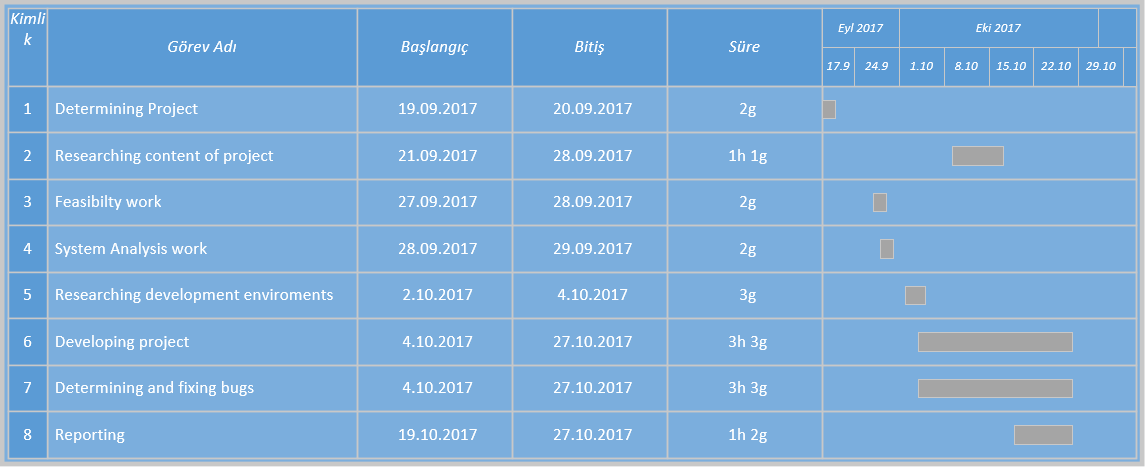
\includegraphics[width=\textwidth]{projectChapters/images/gantt.png}
\caption{Gantt Diyagramı Zaman Çizelgesi}
\end{figure}


\section{Legitimate Feasibility}
Software which is used within the project does not face any legal issues. All of the
software used in the project contain license requirements. Users are responsible for
all shared content. The users are responsible of their well being. So any misusing of 
any sharing content is their risk. So sharing and publishing content is on their own risk.


\section{Economic Feasibility}
There is no charge for software components to be used during application development. The hourly working fee of the person who will develop the project is 25 TL per person. The total cost determined for the project during the project development period stated in the Gantt Chart is 8000 TL. The price of a computer with minimum system requirements stated in the title of hardware feasibility which costs currently between 1500 and 2500 TL. Price of Google Map API is 4\$ and 15 TL per month. Price of AWS is 15\$ and 60 TL per month.

\begin{table}[]
\centering
\caption{Total Cost Table For Gezi-Yorum}
\label{my-label}
\begin{tabular}{|l|l|}
\hline
\multicolumn{1}{|c|}{\textbf{Cost}} & \multicolumn{1}{c|}{\textbf{TL}} \\ \hline
Hardware                               & 5.000,00 TL                      \\ \hline
Project Team                           & 16.000,00 TL                      \\ \hline
Google Map API                         & 15,00 TL                      \\ \hline
AWS                                 & 60,00 TL                      \\ \hline
\textbf{Toplam}                        & \textbf{21.075,00 TL}            \\ \hline
\end{tabular}
\end{table}




